\documentclass[aspectratio=169, 10pt]{beamer}

% --- Packages ---
\usepackage[utf8]{inputenc}
\usepackage[T1]{fontenc}
\usepackage{helvet} % Use Helvetica for a cleaner, modern look
\usepackage{tcolorbox}
\usepackage{tikz}
\usepackage{amsmath}
\usepackage{graphicx}
\usepackage{hyperref}

% --- Theme & Aesthetics ---
\usetheme{Madrid}
\useinnerchannel{rectangles}
\useoutertheme{infolines}

% Custom Colors (Premium Quantum Theme)
\definecolor{QuantumDeepBlue}{HTML}{0F172A} % Dark background
\definecolor{QuantumPurple}{HTML}{7C3AED}   % Primary accent
\definecolor{QuantumCyan}{HTML}{06B6D4}     % Secondary accent
\definecolor{QuantumLight}{HTML}{F1F5F9}    % Text color
\definecolor{QuantumGray}{HTML}{334155}     % Block background

% Apply Colors
\setbeamercolor{palette primary}{bg=QuantumDeepBlue,fg=white}
\setbeamercolor{palette secondary}{bg=QuantumPurple,fg=white}
\setbeamercolor{palette tertiary}{bg=QuantumDeepBlue,fg=white}
\setbeamercolor{palette quaternary}{bg=QuantumCyan,fg=QuantumDeepBlue}
\setbeamercolor{structure}{fg=QuantumCyan} % Itemize, frames, etc.

\setbeamercolor{background canvas}{bg=white} % clean white background for readability, or use dark? Let's stick to white for printability/standard, but with dark headers.
% Actually, for "Premium", let's do a slight off-white bg and dark headers.

\setbeamercolor{title}{bg=QuantumDeepBlue,fg=white}
\setbeamercolor{frametitle}{bg=QuantumDeepBlue,fg=white}
\setbeamercolor{block title}{bg=QuantumPurple,fg=white}
\setbeamercolor{block body}{bg=QuantumLight!50!white,fg=black}

% Font adjustments
\setbeamerfont{title}{size=\huge,series=\bfseries}
\setbeamerfont{frametitle}{size=\Large,series=\bfseries}

% --- Metadata ---
\title[Hardware-Efficient VQE]{Hardware-efficient Variational Quantum Eigensolver\\for Small Molecules and Quantum Magnets}
\subtitle{Replikasi dan Penjelasan Paper}
\author{Tim Replikasi}
\institute[DreamyTA]{DreamyTA Project}
\date{\today}

\begin{document}

% --- Slide 1: Judul ---
\begin{frame}
    \titlepage
    \begin{center}
        \textit{\small Based on work by IBM Quantum Team (Kandala et al.)}
    \end{center}
\end{frame}

% --- Bagian 1: Pendahuluan ---
\section{Pendahuluan \& Motivasi}

% --- Slide 2: Masalah Utama ---
\begin{frame}{Masalah Utama: Struktur Elektronik}
    \begin{columns}
        \column{0.5\textwidth}
        \begin{block}{Tujuan}
            Menentukan \textbf{Energi Keadaan Dasar} (\textit{Ground State Energy}) molekul.
            $$ H |\Psi\rangle = E |\Psi\rangle $$
        \end{block}
        \vspace{0.5em}
        \begin{itemize}
            \item Sifat kimia material bergantung pada interaksi elektron (fermion).
            \item \textbf{Tantangan Klasik:} Biaya komputasi berskala \textbf{eksponensial}.
            \item \textit{Monte Carlo} gagal karena \textbf{Fermionic Sign Problem}.
        \end{itemize}

        \column{0.5\textwidth}
        \centering
        % Placeholder for molecule illustration
        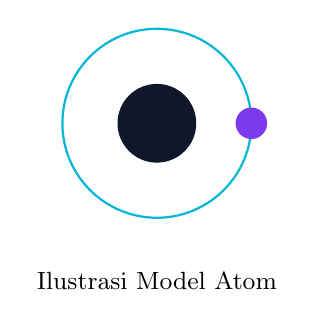
\begin{tikzpicture}
            \fill[QuantumDeepBlue] (0,0) circle (0.5);
            \draw[thick, QuantumCyan] (0,0) circle (1.2);
            \fill[QuantumPurple] (1.2,0) circle (0.2);
            \node at (0,-2) {\small Ilustrasi Model Atom};
        \end{tikzpicture}
    \end{columns}
\end{frame}

% --- Slide 3: Mengapa Komputer Kuantum? ---
\begin{frame}{Mengapa Komputer Kuantum? \& Tantangannya}
    \begin{alertblock}{Janji Komputer Kuantum}
        Komputer kuantum secara alami cocok untuk mensimulasikan sistem kuantum (Feynman).
    \end{alertblock}

    \vspace{1em}

    \begin{columns}
        \column{0.48\textwidth}
        \begin{tcolorbox}[colback=green!10!white, colframe=green!50!black, title=Teori (Quantum Phase Estimation)]
            \begin{itemize}
                \item Bisa memberikan hasil eksak.
                \item Algoritma "Buku Teks".
            \end{itemize}
        \end{tcolorbox}
        
        \column{0.48\textwidth}
        \begin{tcolorbox}[colback=red!10!white, colframe=red!50!black, title=Realita (NISQ)]
            \begin{itemize}
                \item Sirkuit terlalu panjang (Deep).
                \item Waktu koherensi pendek (Noise).
                \item \textbf{QPE Gagal} di hardware saat ini.
            \end{itemize}
        \end{tcolorbox}
    \end{columns}
    
    \vspace{1em}
    \centering
    \textbf{Solusi:} Kita butuh algoritma yang "tahan banting" dengan sirkuit pendek.
\end{frame}

% --- Bagian 2: Metodologi ---
\section{Metodologi (Solusi)}

% --- Slide 4: VQE ---
\begin{frame}{Solusi Hibrida: VQE (Variational Quantum Eigensolver)}
    \begin{center}
        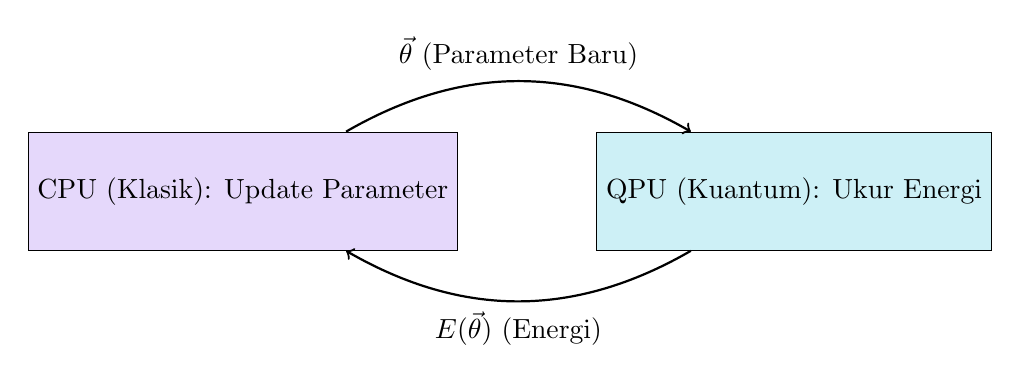
\begin{tikzpicture}[node distance=3cm, auto]
            \node [draw, fill=QuantumPurple!20, rectangle, minimum height=1.5cm] (cpu) {CPU (Klasik): Update Parameter};
            \node [draw, fill=QuantumCyan!20, rectangle, minimum height=1.5cm, right of=cpu, node distance=7cm] (qpu) {QPU (Kuantum): Ukur Energi};
            
            \draw [->, thick, bend left] (cpu) to node { $\vec{\theta}$ (Parameter Baru)} (qpu);
            \draw [->, thick, bend left] (qpu) to node { $E(\vec{\theta})$ (Energi)} (cpu);
        \end{tikzpicture}
    \end{center}

    \vspace{1em}
    \begin{itemize}
        \item \textbf{Algoritma Hibrida:} Membagi tugas antara komputer klasik dan kuantum.
        \item \textbf{Prinsip Variasional Ritz:} 
        $$ \langle \Psi(\theta) | H | \Psi(\theta) \rangle \ge E_{ground} $$
        Kita hanya perlu meminimalkan energi tebakan kita.
    \end{itemize}
\end{frame}

% --- Slide 5: Masalah Ansatz Standar ---
\begin{frame}{Masalah pada Ansatz Standar (UCC)}
    \begin{block}{Unitary Coupled Cluster (UCC)}
        Metode "Emas" di Kimia Komputasi, sangat akurat namun...
    \end{block}

    \begin{itemize}
        \item[\textbf{X}] \textbf{Mahal:} Jumlah gerbang meledak secara polinomial.
        \item[\textbf{X}] \textbf{Trotterisasi:} Membutuhkan pemotongan langkah waktu $\rightarrow$ Sirkuit menjadi sangat dalam.
        \item[\textbf{X}] \textbf{Akibat:} Noise menghancurkan hasil sebelum perhitungan selesai.
    \end{itemize}

    \vspace{1em}
    \centering
    \textit{Penulis memutuskan untuk \textbf{TIDAK} menggunakan UCC demi efisiensi hardware.}
\end{frame}

% --- Slide 6: Hardware Efficient Ansatz ---
\begin{frame}{Inovasi: Hardware-Efficient Ansatz}
    \begin{columns}
        \column{0.6\textwidth}
        \textbf{Ide Inti:} Jangan paksakan rumus kimia ke hardware. Sesuaikan tebakan (\textit{ansatz}) dengan gerbang alami chip.
        
        \vspace{1em}
        \textbf{Komponen Sirkuit:}
        \begin{enumerate}
            \item \textbf{Rotasi Euler (Single-Qubit):} $U_{q,i}(\theta)$ untuk kontrol.
            \item \textbf{Entangler ($U_{ENT}$):} Menggunakan \textit{Drift Hamiltonian} (interaksi alami).
        \end{enumerate}
        
        \column{0.4\textwidth}
        \begin{tcolorbox}[title=Keunggulan]
            \begin{itemize}
                \item Sirkuit Pendek (Shallow).
                \item Minim akumulasi error.
                \item Tidak butuh kalibrasi CNOT sempurna.
            \end{itemize}
        \end{tcolorbox}
    \end{columns}
\end{frame}

% --- Bagian 3: Implementasi ---
\section{Implementasi Eksperimental}

% --- Slide 7: Peta Jalan ---
\begin{frame}{Peta Jalan Eksperimen (Overview)}
    \begin{columns}
        \column{0.5\textwidth}
        \textbf{1. Mapping (Kimia $\rightarrow$ Qubit)}
        \begin{itemize}
            \item Parity Mapping.
            \item Reduksi Qubit (misal: 8 orbital $\rightarrow$ 6 qubit).
        \end{itemize}
        
        \vspace{1em}
        \textbf{2. Hardware (The Chip)}
        \begin{itemize}
            \item Prosesor 7-Qubit (Pakai 6).
            \item Konektivitas terbatas (\textit{waveguide}).
        \end{itemize}

        \column{0.5\textwidth}
        \textbf{3. Sirkuit (The Ansatz)}
        \begin{itemize}
            \item Berlapis (Layered).
            \item Depth $d$: Jumlah pengulangan $U_{ENT}$.
        \end{itemize}

        \vspace{1em}
        \textbf{4. Fisik (Pulse)}
        \begin{itemize}
            \item Sinyal Mikrogelombang.
            \item Cross-Resonance Gate.
        \end{itemize}
    \end{columns}
\end{frame}

% --- Slide 8: Optimasi SPSA ---
\begin{frame}{Strategi Optimasi: SPSA}
    \begin{block}{Tantangan Pengukuran}
        Pengukuran kuantum bersifat probabilistik (berisik/fluktuasi). Metode gradien biasa butuh terlalu banyak sampel.
    \end{block}

    \vspace{0.5em}
    \textbf{Solusi: SPSA (Simultaneous Perturbation Stochastic Approximation)}
    \begin{itemize}
        \item Mengestimasi gradien hanya dengan \textbf{2 pengukuran}.
        \item Tidak peduli jumlah parameter (mau 10 atau 100, tetap 2 pengukuran).
        \item Sangat hemat waktu dan cocok untuk lingkungan ber-noise.
    \end{itemize}

    \vspace{1em}
    \centering
    \textit{Grafik konvergensi energi biasanya terlihat bergerigi di awal, lalu melandai.}
\end{frame}

% --- Bagian 4: Hasil ---
\section{Hasil \& Diskusi}

% --- Slide 9: Hasil BeH2 ---
\begin{frame}{Hasil Puncak: Molekul BeH2 (6 Qubit)}
    \begin{columns}
        \column{0.5\textwidth}
        \begin{itemize}
            \item \textbf{Molekul:} Berilium Dihidrida (BeH2).
            \item \textbf{Skala:} Molekul terbesar yang diuji (6 Qubit).
            \item \textbf{Metode:} Frozen Core Approximation.
        \end{itemize}
        \vspace{1em}
        \textbf{Hasil:}
        \begin{itemize}
            \item Garis hijau (Eksperimen) berhimpitan dengan garis hitam (Teori).
            \item \textit{Chemical Accuracy} tercapai dengan depth $d=1$ dan 30 parameter.
        \end{itemize}

        \column{0.5\textwidth}
        \centering
        \textbf{[Visual: Grafik Energi vs Iterasi BeH2]}
        \vspace{3cm} % Placeholder space
    \end{columns}
\end{frame}

% --- Slide 10: Kurva Energi Potensial ---
\begin{frame}{Kurva Energi Potensial: H2, LiH, BeH2}
    Eksperimen diulang pada berbagai jarak antar-atom.
    \vspace{1em}
    
    \begin{columns}
        \column{0.33\textwidth}
        \centering
        \textbf{H2 (2 Qubit)}
        \vspace{0.5em}
        \begin{itemize}
            \item Sangat Akurat.
            \item $d=1$ Sudah Cukup.
        \end{itemize}

        \column{0.33\textwidth}
        \centering
        \textbf{LiH (4 Qubit)}
        \vspace{0.5em}
        \begin{itemize}
            \item Ada penyimpangan di 2.5 \AA.
            \item Sebab: Sirkuit $d=1$ kurang dalam (\textit{Underfitting}).
            \item Trade-off: Tambah $d$ = Tambah Noise.
        \end{itemize}

        \column{0.33\textwidth}
        \centering
        \textbf{BeH2 (6 Qubit)}
        \vspace{0.5em}
        \begin{itemize}
            \item Mengikuti tren teori.
            \item Pembuktian skalabilitas metode.
        \end{itemize}
    \end{columns}
\end{frame}

% --- Slide 11: Validasi Noise ---
\begin{frame}{Validasi Noise (Simulasi vs Eksperimen)}
    \begin{tcolorbox}[colback=QuantumLight, colframe=QuantumDeepBlue, title=Pemahaman Error]
        Grafik paper menunjukkan \textbf{shaded region} (area berwarna).
    \end{tcolorbox}
    
    \begin{itemize}
        \item \textbf{Shaded Region:} Hasil simulasi klasik yang \textit{sengaja} diberi noise ($T_1, T_2$, sampling error).
        \item \textbf{Observasi:} Data eksperimen jatuh tepat di dalam area tersebut.
        \item \textbf{Kesimpulan:} Error pada eksperimen sudah diprediksi dan dipahami dengan baik. Tidak ada anomali tak terjelaskan.
    \end{itemize}
\end{frame}

% --- Slide 12: Magnetisme ---
\begin{frame}{Bonus: Aplikasi Magnetisme (Heisenberg Model)}
    \textit{Metode ini fleksibel, tidak hanya untuk kimia.}
    
    \vspace{1em}
    \textbf{Kasus: Model Heisenberg Antiferomagnetik ($J$ vs $B$)}
    
    \begin{columns}
        \column{0.5\textwidth}
        \begin{block}{Dominasi Medan Luar ($B \gg J$)}
            \begin{itemize}
                \item Qubit cenderung mandiri.
                \item Sirkuit $d=0$ (Tanpa Entangler) menang.
            \end{itemize}
        \end{block}

        \column{0.5\textwidth}
        \begin{block}{Dominasi Interaksi ($J \gg B$)}
            \begin{itemize}
                \item Qubit sangat \textit{entangled}.
                \item Wajib pakai sirkuit $d=2$.
                \item $d=0$ gagal total.
            \end{itemize}
        \end{block}
    \end{columns}
\end{frame}

% --- Bagian 5: Kesimpulan ---
\section{Kesimpulan}

% --- Slide 13: Kesimpulan ---
\begin{frame}{Kesimpulan & Masa Depan}
    \begin{enumerate}
        \item \textbf{Pencapaian Besar:} Berhasil mensimulasikan molekul BeH2 (6 Qubit) pada perangkat NISQ tanpa \textit{Error Correction}.
        \item \textbf{Resep Sukses:}
        $$ \text{VQE} + \text{Hardware-Efficient Ansatz} + \text{SPSA} $$
        \item \textbf{Tantangan Masa Depan (Skalabilitas):}
        \begin{itemize}
            \item Butuh konektivitas qubit yang lebih baik.
            \item Butuh waktu koherensi lebih panjang (untuk $d$ lebih dalam).
        \end{itemize}
    \end{enumerate}
    
    \vspace{1em}
    \centering
    \large \textbf{"Paper ini membuktikan bahwa komputer kuantum jangka pendek bisa berguna untuk masalah sains nyata."}
\end{frame}

% --- Slide 14: Q&A ---
\begin{frame}
    \centering
    \Huge \textbf{Terima Kasih}
    
    \vspace{1em}
    \Large Sesi Tanya Jawab
    
    \vspace{2em}
    \normalsize
    \textit{Tim Replikasi DreamyTA}
\end{frame}

\end{document}
